\titlespacing*{\subsection}
  {0pt}{2\baselineskip}{\baselineskip}

\part{Informática}

\chapter{Métodos de muestreo directo de fuentes de luz}\label{MuestreoDirecto}
Una característica común a todos los algoritmos de aproximación de la ecuación de renderización es que eventualmente tendrán que muestrear las direcciones que apuntan hacia las fuentes de luz de la escena con el objetivo de utilizar estas muestras para evaluar el correspondiente estimador de Monte Carlo.

Supongamos que queremos aproximar la integral de una función $g_P:\mathds{S}^2\rightarrow \mathds{R}_0^+$ sobre el ángulo sólido subtendido por una fuente de luz desde un punto $P$ de la escena. Usualmente tendremos:
$$g_P(\omega) = L_e(t(P,\omega), -\omega)f(P,\omega_o,\omega)\cos(n(P),\omega),$$

para alguna dirección $\omega_o$, donde $t$ es la función que asigna a cada pareja $(x,\omega)$ el primer punto visible desde $x$ en dirección $\omega$ y $n(P)$ es la normal a la superficie en $P$. Para estimar dicha integral utilizando un estimador Monte Carlo necesitamos ser capaces de tomar muestras respecto de alguna distribución de probabilidad definida sobre el ángulo sólido subtendido por la fuente de luz.

Como ya se ha mencionado anteriormente, la forma más sencilla de muestrear una fuente de luz de área es generar una muestra con distribución uniforme en su superficie y obtener la función de densidad de la muestra respecto al ángulo sólido, teniendo en cuenta la transformación \ref{cambioArea}. Sin embargo, cuando la fuente de luz está muy cerca del punto $P$, este método de muestreo puede llevar a una varianza muy alta. En efecto, vemos que:
$$E[\frac{g_P(\omega)^2}{f_{\omega}(\omega)^2}] = \int \frac{g_P(\omega)^2}{f_{\omega}(\omega)} d\mu(\omega) = \int \frac{g_P(\omega)^2A_F \cos(n(t(P,\omega)),\omega)}{\|t(P,\omega)-P\|^2} d\mu(\omega),$$

donde $A_F$ es el área de la fuente de luz y $f_{\omega}$ es la función de densidad asociada al método de muestreo uniforme respecto al área. Recordando la discusión en \ref{MI}, cuando $\|t(P,\omega)-P\|$ sea cercano a $0$, o lo que es lo mismo, cuando la fuente de luz esté muy cerca de $P$, $E[\frac{g_P(\omega)^2}{f_{\omega}(\omega)^2}]$ alcanzará valores altos, y por tanto la varianza del estimador Monte Carlo de la función $\frac{g_P}{f_{\omega}}$ será muy alta. Que la varianza sea alta implicará que necesitaremos más muestras por píxel para acercarnos al valor real, y esto a su vez incrementará el tiempo de ejecución necesario para generar la imagen final. 

En este capítulo presentaremos e implementaremos una serie de algoritmos de muestreo de fuentes de luz, alternativos al muestreo uniforme respecto al área, que pretenden reducir la varianza del estimador de Monte Carlo. Los algoritmos serán implementados en el renderizador fotorrealista de código libre asociado descrito en el libro (), que es accesible a través de \href{https://github.com/mmp/pbrt-v3}{este} enlace. 

\section{Muestreo uniforme de rectángulos esféricos}

En esta sección presentaremos un método de muestreo para fuentes de luz rectangulares, descrito en \cite{Urena2013}. Se denomina rectángulo esférico a la proyección de un rectángulo sobre una esfera unidad. Fijado un punto $P\in\mathds{R}^3$ de la escena, consideramos $\pi_P$ la proyección sobre la esfera unidad con centro $P$. Dada una fuente de luz rectangular $F$, nuestro objetivo es tomar muestras en el rectángulo esférico $\pi_P(F)$ utilizando una distribución uniforme respecto al ángulo sólido, esto es, una distribución cuya función de densidad asociada cumpla que:
$$f_{\omega}(\omega) = \frac{1}{\mu(\pi_P(F))}\text{, }\forall \omega\in\pi_P(F)$$

Con este objetivo describiremos una parametrización $M:[0,1]^2\rightarrow \pi_P(F)$ que preserva el área. Cuando decimos que preserva el área queremos decir que para cualquier subconjunto $U\subseteq [0,1]^2$ se cumple que:
$$\frac{\mu(M(U))}{\mu(\pi_P(F))} = A(U)$$

donde $A(U)$ es el área del conjunto $U$. Por el teorema del cambio de variable, tenemos que:
$$\mu(\pi_P(F))A(U) = \mu(M(U)) = \int_{M(U)}d\omega = \int_{U}|det(J_M(x,y))| dxdy $$

y dado que la igualdad anterior se da para todo $U\subseteq [0,1]^2$, deducimos que el mapa $M$ preserva el área si y solo si $|det(J_M(x,y))| = \mu(\pi_P(F))$ para todo $(x,y)\in[0,1]^2$. En vista de esta propiedad, si $V$ es un vector aleatorio con distribución uniforme en $[0,1]^2$, entonces la función de densidad de $M(V)$ cumple que:
$$f_{M(V)}(M(v)) = \frac{f_V(v)}{|det(J_M(v))|}\Rightarrow f_{M(V)}(M(v)) =\frac{1}{\mu(\pi_P(F))} \text{, }\forall v\in [0,1]^2$$

Concluimos que basta aplicar el mapa $M$ a una muestra siguiendo la distribución uniforme en $[0,1]^2$ para obtener una muestra siguiendo la distribución uniforme en $\pi_P(F)$. Pasamos por tanto a describir el mapa $M$.\\

\begin{figure}[h]
  \lineskip=-\fboxrule
  \fbox{\begin{minipage}{\dimexpr \textwidth-2\fboxsep-2\fboxrule}
    \centering
    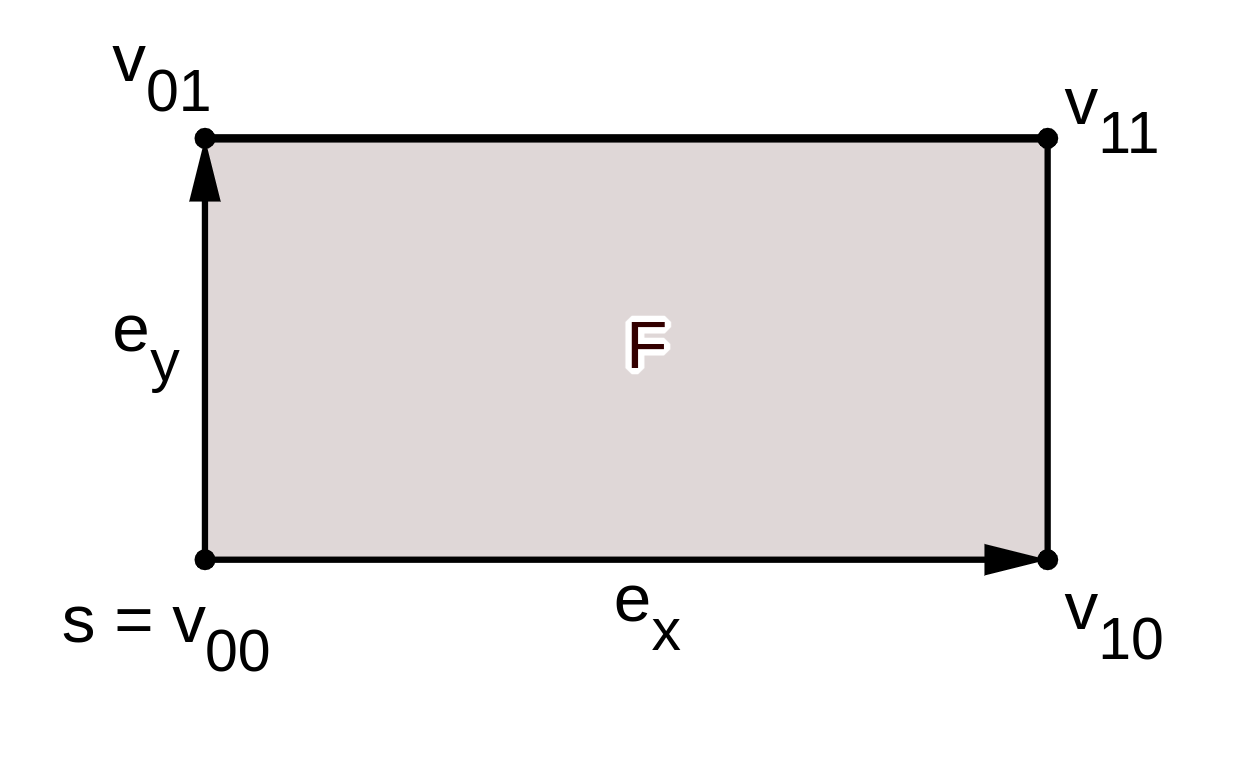
\includegraphics[width=0.6\textwidth]{imagenes/figura4_1}
  \end{minipage}}
  \fbox{\begin{minipage}{\dimexpr \textwidth-2\fboxsep-2\fboxrule}
    \abovecaptionskip=0pt
    \caption{Puntos relevantes de la fuente de luz rectangular $F$.}
  \end{minipage}}
\end{figure}

\subsection{Construcción de la parametrización $M$ }

En primer lugar, describiremos el sistema de referencia en el que vamos a trabajar. Fijemos $P\in\mathds{R}^3$ el punto desde el cual queremos muestrear el ángulo sólido subtendido por el rectángulo $F$. Fijemos un vértice $s$ del rectángulo $F$ y consideremos los dos vectores $e_x$ y $e_y$ cuyo punto inicial es el vértice $s$ y cuyos puntos finales son los vértices adyacentes a $s$ (véase la figura 4.1). Sea $z$ el vector de longitud unidad perpendicular a $e_x$ y $e_y$ tal que $(s-P)\cdot z < 0$. Entonces, notando $x=\frac{e_x}{\|e_x\|}$, $y=\frac{e_y}{\|e_y\|}$, trabajaremos respecto al sistema de referencia $S=\{P; (x, y, z)\}$, por lo que todos los vectores de coordenadas serán respecto a $S$.

Consideramos ahora los siguientes valores:
$$ x_0 = (s-P)\cdot x\hspace{0.5cm}y_0 = (s-P)\cdot y\hspace{0.5cm}z_0 = (s-P)\cdot z$$
$$\hspace{0.5cm}x_1 = x_0+\|e_x\|\hspace{0.5cm}y_1 = y_0+\|e_y\|$$

Notaremos $v_{ij} := (x_i,y_j,z_0)$, $i=0,1$, $j=0,1$, a los cuatro vértices del rectángulo $F$. Consideramos la pirámide con ápide $P$ y base $F$, y tomamos las normales a cada uno de los planos laterales de la pirámide:
$$ n_0 = \frac{v_{00}\times v_{10}}{\|v_{00}\times v_{10}\|}\hspace{0.5cm}n_1 = \frac{v_{10}\times v_{11}}{\|v_{10}\times v_{11}\|}$$
$$ n_2 = \frac{v_{11}\times v_{01}}{\|v_{11}\times v_{01}\|}\hspace{0.5cm}n_3 = \frac{v_{01}\times v_{00}}{\|v_{01}\times v_{00}\|}$$

Notamos por $\gamma_i := \arccos(-n_i\cdot n_{i+1})$, $i=0,1,2$, $\gamma_3 := \arccos(-n_3\cdot n_0)$ al ángulo interior que forman los planos laterales de la pirámide. Se puede demostrar utilizando el teorema de Girard que el ángulo sólido subtendido por $F$ desde $P$ o, equivalentemente, el área de $\pi_P(F)$, mide:
$$\mu(\pi_P(F)) = \gamma_0 +\gamma_1 + \gamma_2 + \gamma_3 - 2\pi $$

Dado que $F$, que es la base de la pirámide descrita, tiene los lados paralelos a los ejes de coordenadas, se cumple que $n_i$ tendrá al menos una coordenada nula para todo $i$. En efecto vemos que existen $\varphi_0,\ldots,\varphi_3$ tales que:
$$ n_0 = \cos(\varphi_0)z + \sin(\varphi_0)y\hspace{0.5cm}n_1 = \cos(\varphi_1)z + \sin(\varphi_1)x$$
$$ n_2 = \cos(\varphi_2)z + \sin(\varphi_2)y\hspace{0.5cm}n_3 = -\cos(\varphi_3)z - \sin(\varphi_3)x$$

Pasamos ya a construir la parametrización $M$ que preserva el área. Tomamos $v=(v_1,v_2)\in [0,1]^2$. Pretendemos encontrar $(x_v,y_v,z_0)$ las coordenadas respecto al sistema de referencia $S$ de un punto en $F$ tal que su proyección sobre la esfera sea igual a $M(v)$. Para calcular $x_v$, establecemos un rectángulo esférico $Q_v$ contenido en $\pi_P(F)$ tal que el área de $Q_v$ cumpla que:
$$\mu(Q_v) = \mu(\pi_P(F)) v_1 $$

Para que $M$ preserve el área tendremos que el rectángulo esférico $Q_v$ es el resultante de proyectar sobre la esfera la parte del rectángulo $F$ que cumple que su primera coordenada es menor o igual que $x_v$. 

\begin{figure}[h]
  \lineskip=-\fboxrule
  \fbox{\begin{minipage}{\dimexpr \textwidth-2\fboxsep-2\fboxrule}
    \centering
    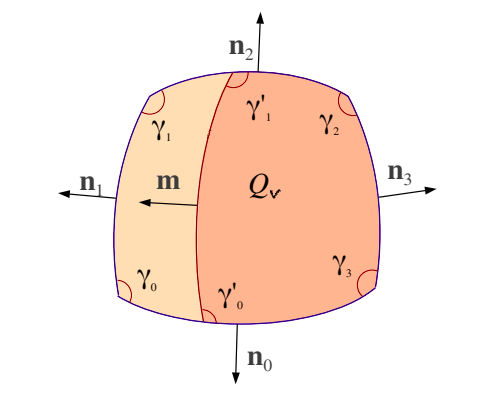
\includegraphics[width=0.6\textwidth]{imagenes/figura4_2}
  \end{minipage}}
  \fbox{\begin{minipage}{\dimexpr \textwidth-2\fboxsep-2\fboxrule}
    \abovecaptionskip=0pt
    \caption{Descripción de los rectángulos esféricos $\pi_P(F)$ y $Q_v$. Imagen extraída de \cite{Urena2013}}
  \end{minipage}}
\end{figure}

Como podemos ver en la figura 4.2, tres de los cuatro planos que delimitan el rectángulo $\pi_P(F)$ también delimitan $Q_v$. El cuarto plano delimitante es el plano que pasa por $P$ y que es perpendicular a cierto vector $m$ perteneciente al plano $y=0$. Por tanto, para algún $\varphi_v$ se tiene que:
$$m=\cos(\varphi_v)z+\sin(\varphi_v)x$$

El ángulo $\varphi_v$ sólo dependerá de $v_1$ y varía desde $\varphi_3$ hasta $\varphi_1$. El área de $Q_v$ cumple que:
\begin{align*}
\mu&(\pi_P(F))v_1 = \mu(Q_v) = \arccos(-n_0\cdot m) +\arccos(-m\cdot n_2) + \gamma_2 +\gamma_3 -2\pi =\\
&= \arccos(-\cos(\varphi_0) \cos(\varphi_v)) +\arccos(-\cos(\varphi_2) \cos(\varphi_v)) + \gamma_2 +\gamma_3 -2\pi 
\end{align*}

Utilizando esta última igualdad y haciendo una serie de derivaciones (ver \cite{Urena2013}) obtenemos que:
$$\cos(\varphi_v) = \frac{\text{sign}(g(v_1))}{\sqrt{g(v_1)^2+\cos(\varphi_0)}}, $$
$$g(v_1) = \frac{\cos(\Phi(v_1))\cos(\varphi_0) - \cos(\varphi_2)}{\sin(\Phi(v_1))}, $$
$$\Phi(v_1) = v_1\mu(\pi_P(F))-\gamma_2-\gamma_3+2\pi$$


\begin{figure}[h]
  \lineskip=-\fboxrule
  \fbox{\begin{minipage}{\dimexpr \textwidth-2\fboxsep-2\fboxrule}
    \centering
    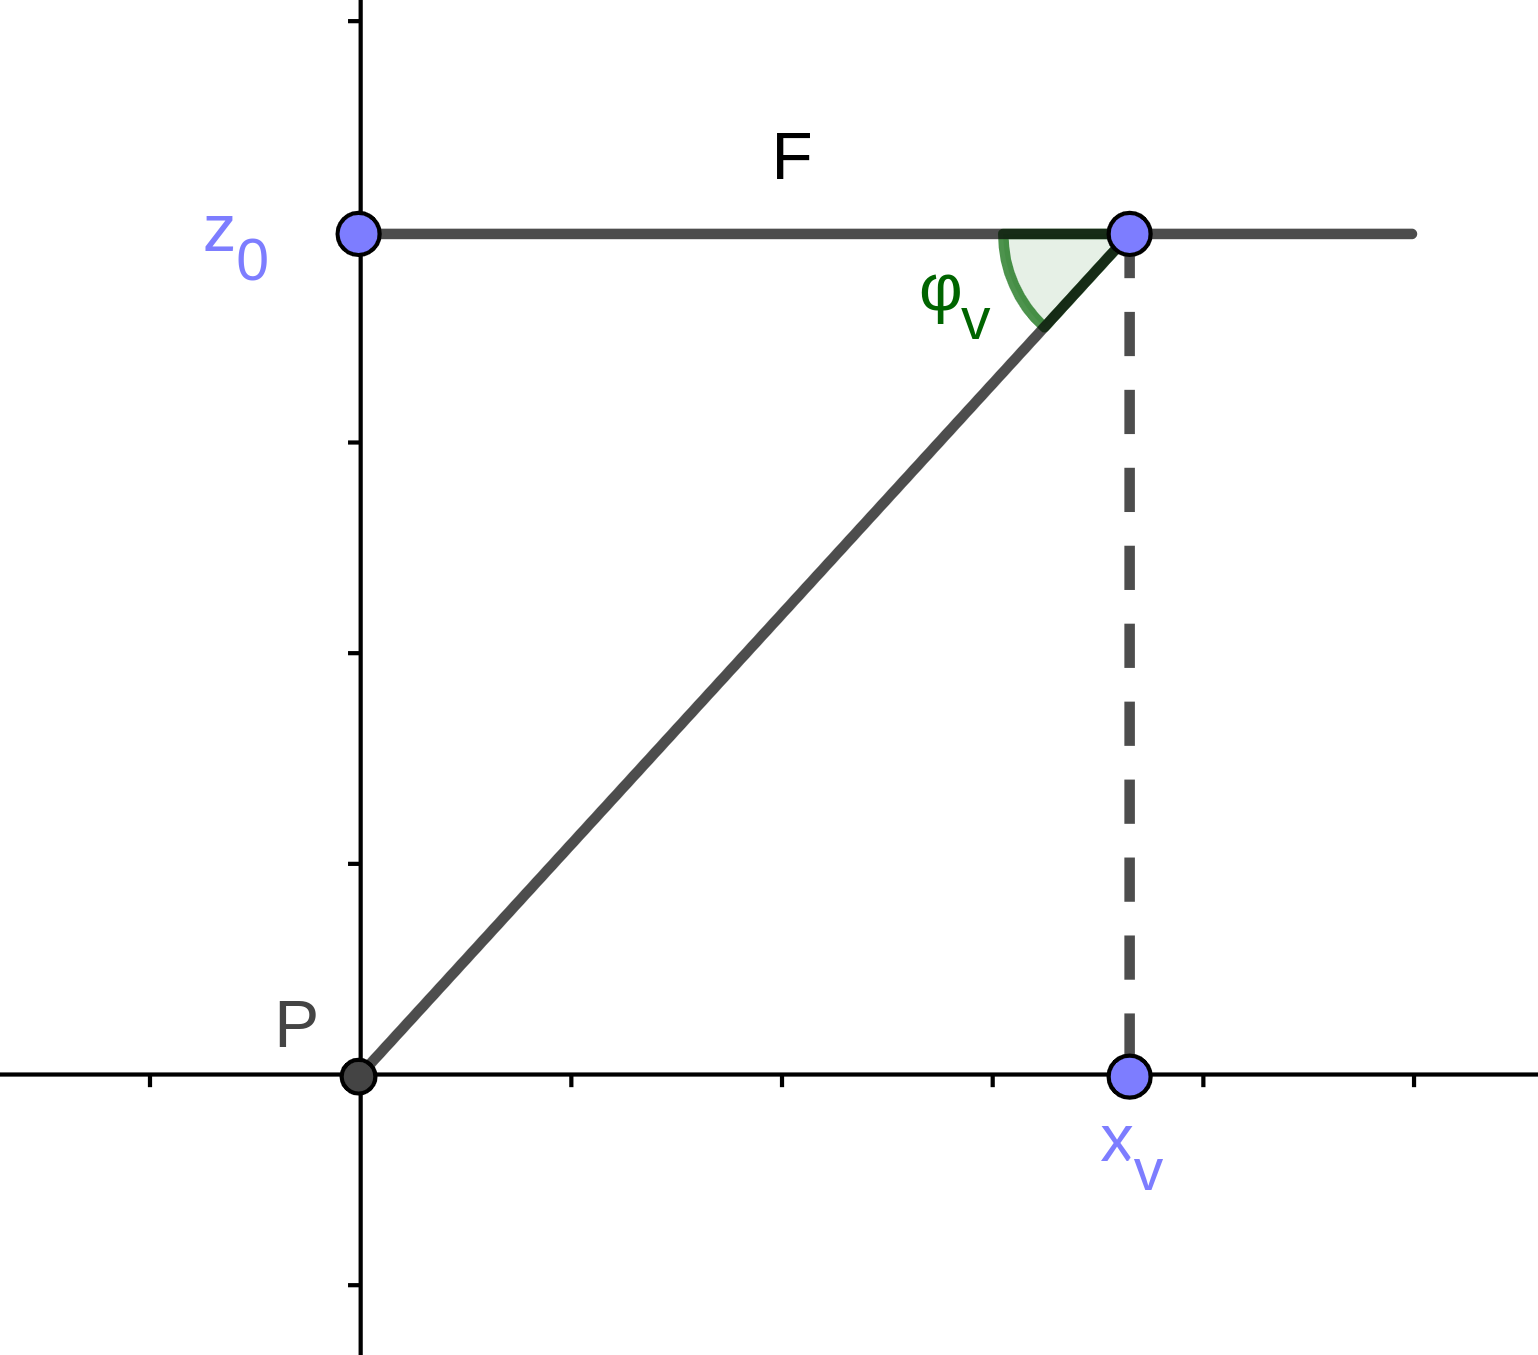
\includegraphics[width=0.6\textwidth]{imagenes/figura4_3}
  \end{minipage}}
  \fbox{\begin{minipage}{\dimexpr \textwidth-2\fboxsep-2\fboxrule}
    \abovecaptionskip=0pt
    \caption{Relación entre $x_v$ y $\varphi_v$}
  \end{minipage}}
\end{figure}

En vista de la figura 4.3, podemos obtener $x_v$ de manera sencilla a partir de $\cos(\varphi_v)$:
$$x_v = -\cos(\varphi_v)\frac{z_0}{\sin(\varphi_v)} = -\cos(\varphi_v)\frac{z_0}{\sqrt{1-\cos(\varphi_v)^2}} $$

Por último, calculemos $y_v$. Ya sabemos que $M(V)$ estará en el segmento:
$$\{(x_v, t y_1 + (1-t) y_0, z_0) / t\in [0,1]\}$$

Para que $M$ preserve el área, en vista de la igualdad \ref{intAngSolSin}, se tiene que cumplir que cambios iguales en $v_2$ generen cambios iguales en $\sin(\theta)$, con $\theta$ el ángulo entre los vectores $y$ y $M(v)$. Para ello, podemos interpolar linealmente la segunda componente de $M(v)$, $h_v$, de la siguiente manera:
$$h_v = h_0 + v_2(h_1-h_0) $$
$$h_0=\frac{y_0}{\sqrt{x_v^2+z_0^2+y_0^2}} $$
$$h_1=\frac{y_1}{\sqrt{x_v^2+z_0^2+y_1^2}}$$

Y concluimos que:
$$y_v = \frac{h_v \sqrt{x_v^2+z_0^2}}{\sqrt{1-h_v^2}}$$

Para finalizar, podemos normalizar el vector $(x_v, y_v, z_0)$, tomando:
$$(\overset{\wedge}{x_v}, h_v, \overset{\wedge}{z_0}) = (x_v, y_v, z_0)\frac{1}{\sqrt{x_v^2 + y_v^2 + z_0^2}}$$

Y tenemos que la dirección $M(v)$ respecto al sistema de referencia usual cumple:
$$M(v) = \overset{\wedge}{x_v} \cdot x + h_v\cdot y + \overset{\wedge}{z_0}\cdot z $$

\subsection{Resultados obtenidos}

\section{Muestreo uniforme de elipses esféricas}

Procedemos de manera similar al caso de fuentes de luz rectangulares. El algoritmo descrito a continuación está recogido en \cite{Guillen2017}. Una elipse esférica es la proyección sobre la esfera unidad de un disco. Consideramos una fuente de luz $D$ cuya superficie es un disco, y fijamos un punto $o\in\mathds{R}^3$ respecto al cual queremos muestrear las direcciones contenidas en la elipse esférica $\pi_o(D)$ siguiendo una distribución uniforme. En este caso construiremos dos parametrizaciones, $M_r:[0,1]^2\rightarrow \pi_o(D)$, $M_s:[0,1]^2\rightarrow \pi_o(D)$, que preservan el área.

\begin{figure}[h]
  \lineskip=-\fboxrule
  \fbox{\begin{minipage}{\dimexpr \textwidth-2\fboxsep-2\fboxrule}
    \centering
    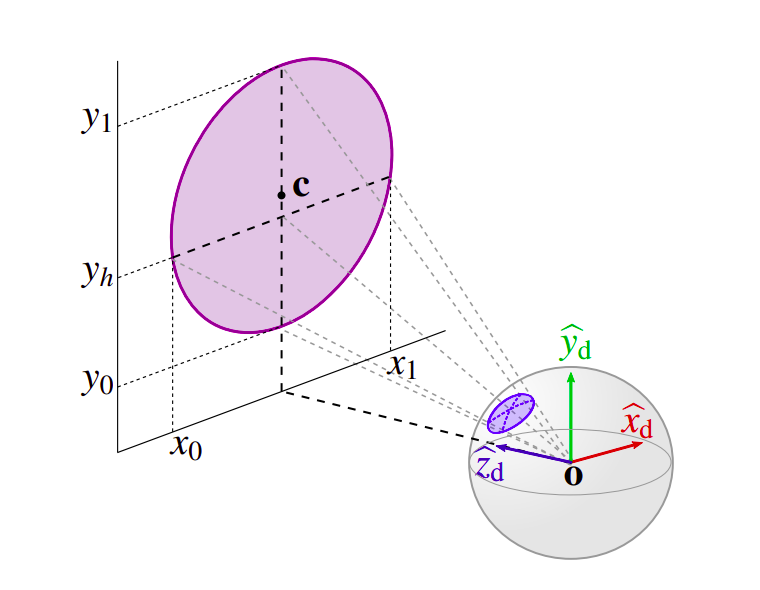
\includegraphics[width=0.6\textwidth]{imagenes/figura4_4}
  \end{minipage}}
  \fbox{\begin{minipage}{\dimexpr \textwidth-2\fboxsep-2\fboxrule}
    \abovecaptionskip=0pt
    \caption{Sistema de referencia y puntos relevantes. Imagen extraída de \cite{Guillen2017}}
  \end{minipage}}
\end{figure}

\subsection{Descripción del sistema de referencia y otros parámetros}

Dada $n_D$ la normal al disco $D$, $c$ el centro del disco $D$, y consideremos los tres siguientes vectores:
$$z_d = -n_D $$
$$x_e = z_d\times \frac{c-P}{\|c-P\|} $$
$$y_d = x_e\times z_d $$

Tomamos el sistema de referencia $S_1=\{o;(x_e, y_d, z_d)\}$ (ver figura 4.4) y todos los vectores de coordenadas aquí descritos serán respecto a $S_1$. Consideramos los puntos $y_0$ e $y_1$ donde el disco toma el valor mínimo y máximo en la segunda coordenada. Si proyectamos $y_0$ e $y_1$ sobre la esfera unidad con centro $o$ obtendremos dos puntos $(0,y_0',z_0')$, $(0,y_1',z_1')$. Entonces el centro de la elipse esférica $\pi_o(D)$ se puede calcular como:
$$z_e = (0,\frac{y_0'+y_1'}{2}, \frac{z_0' + z_1'}{2}) $$

Notar que al reproyectar $z_e$ en el disco obtenemos un punto $(0,y_h,z_h)$ que en general no tiene porque coincidir con el centro del disco $c$. La recta $y = y_h$, $z=z_h$ intersecciona con el disco en dos puntos, $x_0$ y $x_1$. Proyectamos de nuevo el punto $x_1$ sobre la esfera unidad, y consideramos la primera coordenada del punto proyectado, que llamaremos $x_1'$. Por último tomamos los siguientes valores:
\begin{align*}
a = x_1'&\hspace{1cm} b=\frac{1}{2}\sqrt{(y_1'-y_0')^2 + (z_1'-z_0')^2}\\
\alpha = \sin^{-1}(a)&\hspace{1cm} \beta=\sin^{-1}(b)\\
a_t = \tan(\alpha) &\hspace{1cm}b_t=\tan(\beta)
\end{align*}

donde $a$ y $b$ son los semi-ejes de la elipse esférica, $\alpha$ y $\beta$ son sus semi-arcos. Tomando $y_e=z_e\times x_e$, de aquí en adelante cambiaremos el sistema de referencia y trabajaremos sobre $S=\{o;(x_e, y_e, z_e)\}$.

Antes de pasar a describir las dos parametrizaciones, destacar que estas están basadas en el siguiente resultado:

\begin{proposicion}
Sea $\mathds{S}^2$ la esfera unidad de $\mathds{R}^3$, y sea $C$ el cilindro de radio unidad cuyo eje está alineado con el eje $X$. Consideremos la transformación:
$$T:\mathds{S}^2/\{(0,0,1),(0,0,-1)\}\rightarrow C, \hspace{0.7cm} T(x,y,z) = (\frac{x}{\sqrt{x^2+y^2}}, \frac{y}{\sqrt{x^2+y^2}}, z)$$

Entonces dado $A\subseteq\mathds{S}^2$ se cumple que:
$$\int_A dS = \int_{T(A)} dS$$
\end{proposicion}
\begin{proof}
Consideramos la parametrización $\Theta:[0,\pi ]\times [0,2\pi ]\rightarrow \mathds{S}^2$, con:
$$\Theta(\theta ,\varphi ) = ( \sin \theta \cos \varphi,  \sin \theta \sin \varphi , \cos \theta),\hspace{0.5cm}  \forall (\theta , \varphi)\in [0,\pi ]\times [0,2\pi ]$$

Consideramos también la parametrización $\Psi:[0,2\pi ]\times [-1,1]\rightarrow C$, con:
$$\Psi(\varphi , z ) = (\cos \varphi,  \sin \varphi , z),\hspace{0.5cm}  \forall (\varphi, z)\in [0,2\pi ]\times [-1,1]$$

Por la igualdad \ref{intAngSolSin}, y haciendo un sencillo cálculo, vemos que:
$$\int_A dS = \int_{\Theta^{-1}(A)} \sin\theta d\theta d\varphi$$
$$\int_{T(A)} dS = \int_{\Psi^{-1}(T(A))} d\varphi dz $$

Consideramos la función:
$$R:[0,\pi]\times [0,2\pi]\rightarrow [0,2\pi]\times [-1,1] \text{, } R(\theta,\varphi) = (\varphi, \cos(\theta))$$

que cumple que $|det(J_R(\theta,\varphi))| = \sin(\theta)$. Por tanto, aplicando el teorema de cambio de variable, basta ver que $R(\Theta^{-1}(A)) = \Psi^{-1}(T(A))$ para deducir el resultado buscado, lo cuál se deduce fácilmente.
\end{proof}

Este resultado nos dice que el ángulo sólido subtendido por una región de la esfera unidad es igual que el área de esa región proyectada sobre el cilindro de radio uno tal que su eje está alineado con un radio de la esfera.

\subsection{Construcción de la parametrización $M_r$}
Partimos de una muestra $v=(v_1,v_2)\in[0,1]^2$, y vamos a describir como se obtiene la dirección $M_r(v)$ a partir de $v$. En este caso consideramos el cilindro de radio unidad cuyo eje está alineado con $z_e$. Nos centraremos sólo en el caso de muestrear el primer cuadrante de la elipse, haciendo uso del hecho de que la elipse es radialmente simétrica. Para muestrear la elipse completa, basta dividir $[0,1]$ en cuatro intervalos, un intervalo por cada cuadrante, y cambiar el sentido de $x_e$ o $y_e$ convenientemente en función del intervalo al que pertenece $v_1$. Tras hacer esto hay que transformar $v_1$ de manera que el intervalo al que pertenece cubra todo $[0,1]$.

\begin{figure}[h]
  \lineskip=-\fboxrule
  \fbox{\begin{minipage}{\dimexpr \textwidth-2\fboxsep-2\fboxrule}
    \centering
    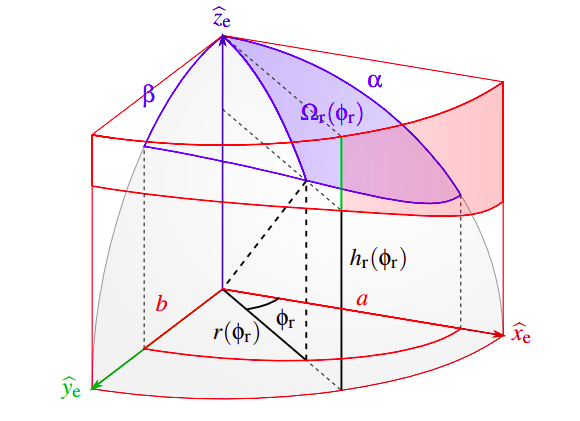
\includegraphics[width=0.6\textwidth]{imagenes/figura4_5}
  \end{minipage}}
  \fbox{\begin{minipage}{\dimexpr \textwidth-2\fboxsep-2\fboxrule}
    \abovecaptionskip=0pt
    \caption{Descripción del mapa $M_r$. Imagen extraída de \cite{Guillen2017}}
  \end{minipage}}
\end{figure}

Observando la figura 4.5, consideramos la función $\Omega_r:[0,\pi /2]\rightarrow \mathds{R}_0^+$ que a cada ángulo $\phi_r$ respecto al eje $x_e$ le asigna el ángulo sólido subtendido por la región azul de la elipse, o lo que es lo mismo, el área de la región roja del cilindro. Está claro que entonces $\mu(\pi_o(D)) = 4\Omega_r(\frac{\pi}{2})$. Es sencillo ver que:
$$\Omega_r(\phi_r)=\int_0^{\phi_r}[1-h_r(x)] dx$$

donde $h_r$ es la función que asigna a cada ángulo $\phi$ respecto al eje $x_e$ la componente $z_e$ del punto más bajo de la línea verde que delimita la región roja. Mediante una serie de derivaciones llegamos a:
$$\Omega_r(\phi_r) = \phi_r -\frac{b(1-a^2)}{a\sqrt{1-b^2}}\Pi(n;\varphi_r|m) $$

donde
$$\Pi(n;\varphi_r|m) = \int_{0}^{\varphi_r}\frac{dx}{(1-n\sin^2(x))\sqrt{1-m\sin^2(x)}}$$

es la integral elíptica incompleta de Legendre y donde
$$n = \frac{a^2-b^2}{a^2(1-b^2)}\hspace{1cm} m=\frac{a^2-b^2}{1-b^2} \hspace{1cm} \varphi_r=\arctan(\frac{a_t}{b_t}\tan(\phi_r))$$

Dado que $\Omega_r$ no se puede invertir analíticamente, podemos utilizar el método de Newton-Raphson para encontrar $\phi_v$ cumpliendo que:
$$\Omega_r(\phi_v)-v_1\Omega_r(\pi/2) = 0 $$

Tomamos ahora $h = (1-v_2)h_r(\phi_v) + v_2$, y podemos definir $M_r(v)$ respecto al sistema de referencia usual como:
$$M_r(v) = \cos(\phi_v)\sqrt{1-h^2}\cdot x_e +\sin(\phi_v)\sqrt{1-h^2}\cdot y_e +h\cdot z_e$$

En efecto, $M_r$ preserva el área.

\subsection{Construcción de la parametrización $M_p$}

\begin{figure}[h]
  \lineskip=-\fboxrule
  \fbox{\begin{minipage}{\dimexpr \textwidth-2\fboxsep-2\fboxrule}
    \centering
    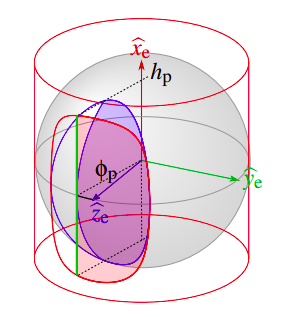
\includegraphics[width=0.5\textwidth]{imagenes/figura4_6}
  \end{minipage}}
  \fbox{\begin{minipage}{\dimexpr \textwidth-2\fboxsep-2\fboxrule}
    \abovecaptionskip=0pt
    \caption{Descripción del mapa $M_p$. Imagen extraída de \cite{Guillen2017}}
  \end{minipage}}
\end{figure}

En este caso, consideramos el cilindro cuyo eje está alineado con el eje $x_e$. En este caso, considerando la imagen 5.6, el ángulo $\phi_p$ va desde $-\beta$ a $\beta$, y la integral del sector cuyo ángulo $\phi_p$ está comprendido entre $-\beta$ y $\phi_p$ (zona roja) se puede calcular como sigue:
$$\Omega_p(\phi_p)=\int_{-\beta}^{\phi_p}2h_p(x)dx,$$

donde $(\phi_p, h_p(\phi_p))$, $(\phi_p, -h_p(\phi_p))$ son los extremos del segmento verde. Claramente el ángulo sólido subtendido por la elipse esférica cumple que:
$$\mu(\pi_o(D)) = \Omega_p(\beta)$$

Se puede derivar una expresión de la función $h_p$, obteniendo (ver \cite{Guillen2017}):
$$h_p(\phi_p)=c_t\sqrt{\frac{1-(p+1)\sin^2\phi_p}{1-(mp+1)\sin^2\phi_p}},$$

donde:
$$p=\frac{1}{b_t^2} \hspace{1cm} m=\frac{a_t^2-b_t^2}{a_t^2+1} \hspace{1cm} c_t=\frac{a_t}{\sqrt{1+a_t^2}}.$$

Claramente por simetría la función $h_p$ cumple que $h_p(x) = h_p(-x)$, $\forall x \in [0,\beta]$. Por tanto, tomando $\Omega_p^+(\phi_p)=\int_0^{\phi_p}2h_p(x)dx$, vemos que:
\[ \Omega_p(\phi_p) =
   \begin{cases}
      \Omega_p^+(\beta)+\Omega_p^+(\phi_p) & :\phi_p\geq0 \\
      \Omega_p^+(\beta)-\Omega_p^+(-\phi_p) & :\phi_p <0
   \end{cases}
  \]

Y sustituyendo la expresión de $h_p$ en $\Omega^+$:
$$\Omega_p^+(\phi_p)=\frac{2c_t}{b_t}[(1-n)\Pi(n;\varphi_p|m)-F(\varphi_p|m)],$$

donde $n=-b_t^2$, $\varphi_p=\sin^{-1}(\frac{\tan\phi_p}{b_t})$, $\Pi$ es la integral elíptica incompleta de Lebesgue de tercer tipo y $F$ es la integral incompleta de Lebesgue de primer tipo, es decir:
$$F(\varphi_p | m) = \int_0^{\varphi_p}\frac{dx}{\sqrt{1-m\sin(x)^2}} $$

Procedemos ahora igual que en el apartado anterior. Sea $v=(v_1,v_2)\in[0,1]^2$, utilizamos el algoritmo de Newton-Raphson para encontrar un $\phi_v$ cumpliendo que:
$$\Omega_p(\phi_v)-v_1\Omega_r(\beta) = 0 $$

Tomamos $h = (-1+v_2)h_p(\phi_v) + v_2h_p(\phi_v)$, y podemos definir $M_p(v)$ respecto al sistema de referencia usual como:
$$M_p(v) = h\cdot x_e +\sin(\phi_v)\sqrt{1-h^2}\cdot y_e + \cos(\phi_v)\sqrt{1-h^2}\cdot z_e$$


\subsection{Resultados obtenidos}


\section{Muestreo de casquetes esféricos proyectados}

En esta sección presentaremos un método de muestreo para fuentes de luz esféricas, descrito en \cite{Urena2018}. Considerando la proyección $\rho$ definida en \ref{proyeccionAnguloSolido}, un casquete esférico proyectado es la imagen por $\rho$ de un casquete esférico sobre la esfera unidad. Fijado un punto $o\in\mathds{R}^3$ de la escena, consideramos $\pi_o$ la proyección sobre la esfera unidad con centro $o$. Consideramos también $\rho_o$ que es la proyección $\rho$ respecto a un sistema de referencia cuyo vector $z$ es la normal a la superficie en $P$, $n_o$. Dada una fuente de luz esférica $E$, nuestro objetivo es tomar muestras en el casquete esférico $\pi_o(E)$. Sin embargo, utilizaremos una distribución uniforme en el casquete esférico proyectado $\rho_o(\pi_o(E))$ para generar una muestra y dicha muestra se trasladará a $\pi_o(E)$ a través de $\rho_o^{-1}$. En vista de \ref{cambioProyectado}, concluimos que las muestras $\omega$ generadas según este procedimiento tendrán una función de densidad asociada:
$$f_{\omega}(\omega) = \frac{cos(\omega , n_o)}{A(\rho_o(\pi_o(E)))}\text{, }\forall \omega\in\pi_o(E)$$

donde $A(\rho_o(\pi_o(E)))$ es el área de $\rho_o(\pi_o(E))$. Igual que en los casos anteriores, definiremos dos mapas $M_s:[0,1]^2\rightarrow \rho_o(\pi_o(E))$, $M_t:[0,1]^2\rightarrow \rho_o(\pi_o(E))$ que preserven el área.

\subsection{Descripción del sistema de referencia y otros parámetros}
Consideramos los siguientes tres vectores, con $s$ el centro de la esfera $E$:
$$\overset{\wedge}{z} = n_o\hspace{1cm} y= \frac{(s-o)\times \overset{\wedge}{z}}{\|(s-o)\times \overset{\wedge}{z}\|} \hspace{1cm} x=\overset{\wedge}{z}\times y$$

En el caso en que el centro de la esfera esté en la misma dirección que $\overset{\wedge}{z}$, tomaremos $y$ cualquier vector perpendicular a $\overset{\wedge}{z}$. Consideremos el siguiente punto, que es la proyección de $s$ sobre la esfera unidad de centro $o$:
$$c=\frac{s-o}{\|s-o\|}$$

Y siendo $r$ el radio de la esfera, consideramos los dos siguientes ángulos (ver figura 4.6, izquierda):
$$\alpha = \arcsin(\frac{r}{\|s-o\|}) \hspace{1cm} \overset{\wedge}{\beta}=\arcsin(\overset{\wedge}{z}(c-o))$$

Vemos que $\overset{\wedge}{\beta}\in[-\pi/2,\pi/2]$. En el caso $\overset{\wedge}{\beta}<0$, tomaremos:
$$z = -\overset{\wedge}{z}\hspace{1cm} \beta = -\overset{\wedge}{\beta}$$

Y en caso de que $\overset{\wedge}{\beta}\geq 0$, tomamos:
$$z = \overset{\wedge}{z}\hspace{1cm} \beta = \overset{\wedge}{\beta}$$

El sistema de referencia que usaremos será $\{o;(x,y,z)\}$.

\begin{figure}[h]
  \lineskip=-\fboxrule
  \fbox{\begin{minipage}{\dimexpr \textwidth-2\fboxsep-2\fboxrule}
    \centering
    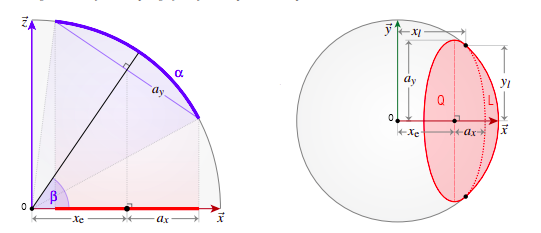
\includegraphics[width=0.9\textwidth]{imagenes/figura4_7}
  \end{minipage}}
  \fbox{\begin{minipage}{\dimexpr \textwidth-2\fboxsep-2\fboxrule}
    \abovecaptionskip=0pt
    \caption{Parametrización de la esfera $Q$ y la luna $L$. Imagen extraída de \cite{Urena2018}}
  \end{minipage}}
\end{figure}

Llegados a este punto tenemos que distinguir dos casos. Por un lado, si $0\leq\alpha\leq\beta$, significará que el casquete esférico $\pi_o(E)$ está completamente contenido en el hemisferio superior de la esfera unidad cuyo polo norte es $z$. En este caso, $\rho_o(\pi_o(E))$ será una elipse. Por otro lado, si $0\leq\beta<\alpha$, el casquete esférico tendrá una parte contenida en el hemisferio superior y otra en el hemisferio inferior. En este caso notaremos por $\rho_o(\pi_o(E))^+$ a la proyección de la parte de $\pi_o(E)$ contenida en el hemisferio superior, que tendrá forma de una elipse $Q$ unida con una luna $L$ (ver figura 4.6 derecha). Notaremos por $\rho_o(\pi_o(E))^-$ a la proyección de la parte de $\pi_o(E)$ contenida en el hemisferio inferior, que tendrá forma de luna $L$.

Vamos por tanto a calcular ciertos parámetros relacionados con la esfera $Q$ y con la luna $L$ (ver figura 4.6 derecha). Por un lado, la longitud de los semiejes de la elipse, $a_x$, $a_y$, y la coordenada $x$ del centro de la elipse, $x_e$, cumplen que:
$$a_y=\sin(\alpha) \hspace{1cm} a_x=\sin(\alpha)\sin(\beta) \hspace{1cm} x_e=\cos(\alpha)\cos(\beta)$$

Por otro lado, en el caso de que $0\leq\beta<\alpha$ y la luna $L$ esté definida, calcularemos los puntos de tangencia de la elipse con el disco, $(x_l,y_l)$, $(x_l,-y_l)$, haciendo uso de que cumplen las ecuaciones de la circunferencia y la elipse, obteniendo que:
$$x_l = \frac{\cos(\alpha)}{\cos(\beta)}\hspace{1cm} y_l=\sqrt{1-\frac{\cos^2(\alpha)}{\cos^2(\beta)}}$$

En el caso de que $0\leq\beta<\alpha$, tenemos que decidir en que hemisferio tomaremos muestras. Dado que partimos de una muestra uniforme en $[0,1]^2$, podemos usar cualquiera de las componentes para determinar que hemisferio muestrearemos, y la probabilidad de muestrear cada uno es proporcional al área relativa entre las dos proyecciones. Si el hemisferio muestreado es el inferior entonces cambiaremos el eje $z$ por $-z$. Una vez determinado el hemisferio muestreado, tenemos que transformar la muestra utilizada para que vuelva a cubrir el intervalo $[0,1]$.

\subsection{Construcción de la parametrización $M_s$}
Por la simetría de los tres tipos de proyección, podemos muestrear sólo en la parte de la proyección con componente $y$ positiva para luego ajustar la muestra en toda la proyección. En vista de la figura 4.7, definimos la siguiente función, que mide el área de una porción de la proyección de la esfera delimitada por un segmento paralelo al eje $x$:
$$A_p(s) = \int_0^s [x_{max}(r)-x_{min}(r)]dr $$

Distinguimos el caso $1$, donde muestreamos solo una elipse $Q$, el caso $2$, donde muestreamos una elipse y una luna, y el caso $3$, donde solo muestreamos la luna $L$. Entonces definimos $x_{max}$ y $x_{min}$ como:
\[ x_{min}(s) = 
   \begin{cases} 
     x_e-a_x\sqrt{1-\frac{s^2}{a_y^2}},  & \text{en el caso $3$}  \\
     x_e+a_x\sqrt{1-\frac{s^2}{a_y^2}},  & \text{en los casos $1$ y $2$}
   \end{cases}
  \]

\[ x_{max}(s) = 
   \begin{cases} 
       x_e+a_x\sqrt{1-\frac{s^2}{a_y^2}},  & \text{si $\alpha\leq\beta$ o si $y_l<s$} \\
       \sqrt{1-s^2}, & \text{si $\beta < \alpha$ y $s\leq y_l$}
   \end{cases}
\]

\begin{figure}[h]
  \lineskip=-\fboxrule
  \fbox{\begin{minipage}{\dimexpr \textwidth-2\fboxsep-2\fboxrule}
    \centering
    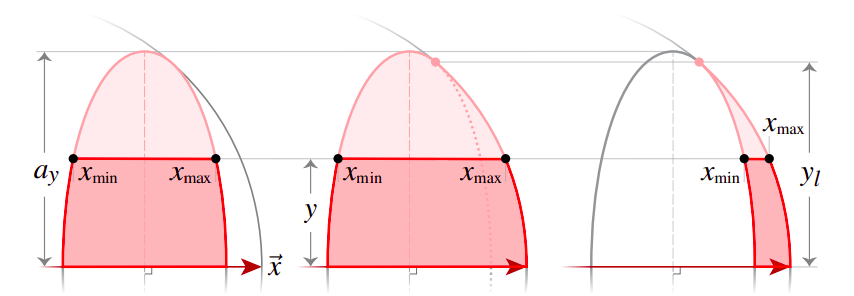
\includegraphics[width=0.9\textwidth]{imagenes/figura4_8}
  \end{minipage}}
  \fbox{\begin{minipage}{\dimexpr \textwidth-2\fboxsep-2\fboxrule}
    \abovecaptionskip=0pt
    \caption{Descripción del mapa $M_s$. Imagen extraída de \cite{Urena2018}}
  \end{minipage}}
\end{figure}

Entonces se cumple que, integrando la expresión anterior:
\[ A_p(s) = 
   \begin{cases} 
       2a_xa_yI(\frac{s}{a_y},1),  & \text{en el caso 1} \\
       2a_xa_yI(\frac{s}{a_y},1) + I(s',1)-x_es' - a_xa_yI(\frac{s'}{a_y},1),  & \text{en el caso 2} \\
       I(s',1)- x_es' -a_xa_yI(\frac{s'}{a_y},1),  & \text{en el caso 3} 
   \end{cases}
\]

con $s'=\min\{y_l,s\}$ y con $I(u,w) = \frac{1}{2}(uw\sqrt{1-u^2} + \arcsin(u))$. Por último tomamos $v=(v_1,v_2)\in[0,1]^2$, y definimos:
\[ y_1 = 
   \begin{cases} 
      y^*: A_p(y^*)-(1-2v_1)A_p(a_y)=0,  & \text{si $v_1<0.5$} \\
      y^*:  A_p(y^*)-(2v_1-1)A_p(a_y)=0,  & \text{si $v_1\geq 0.5$}
   \end{cases}
\]

$$x_1 = x_{min}(y_1) + v_2 (x_{max}(y_1) - x_{min}(y_1))$$

Para calcular el valor de $y_1$, una vez más utilizamos el método de Newton-Raphson. Por último la dirección buscada es:
$$M_s(v) = x_1\cdot x + y_1\cdot y + \sqrt{1-x_1^2-y_1^2} \cdot z.$$

$M_s$ preserva el área por como la hemos construido.

\subsection{Construcción de la parametrización $M_t$}

\begin{figure}[h]
  \lineskip=-\fboxrule
  \fbox{\begin{minipage}{\dimexpr \textwidth-2\fboxsep-2\fboxrule}
    \centering
    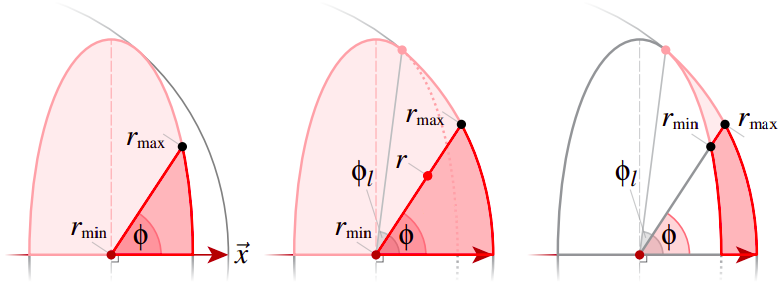
\includegraphics[width=0.9\textwidth]{imagenes/figura4_9}
  \end{minipage}}
  \fbox{\begin{minipage}{\dimexpr \textwidth-2\fboxsep-2\fboxrule}
    \abovecaptionskip=0pt
    \caption{Descripción del mapa $M_t$. Imagen extraída de \cite{Urena2018}}
  \end{minipage}}
\end{figure}

\subsection{Resultados obtenidos}

